% Start with the first chapter
\chapter{Introduction}
% With \label you can define a crossreference so that you can refer
% to this chapter later in the text by using Chapter~\ref{ch:background}
\label{ch:introduction}


Start your introduction here...

Possibly cite some work of others, too \citep{Adiku.ea:1995:USO}. To do so, you have to fill a file (the bibliography, recognisable by the \texttt{.bib} ending) with appropriately formatted references. It would be daft to not use BibDesk or JabRef or other software to manage your references and produce this file for your. Then, you cite the references, and the \textbf{natbib} package allows you flexibility (with/out parentheses, only the year, etc). The actual style of the bibliography in your thesis is determined by the command \texttt{bibliographystyle}, and there are only few defaults. The main differences are between author-year styles (e.g. apalike) and numbered (e.g. ksfh\_nat). Thousands of styles float the internet, recognisable as \texttt{.bst}-files, and typically every journal has a different one, every book series re-invents the styles, and you can spend years optimising what is, essentially, not so super important.

\begin{boxmd}
	\textbf{Bibliography settings}\\
	Just like in any other writing software, references are collected and managed in a dedicated programme (a reference manager, e.g. Zotero, BibDesk, JabRef, ...). This results, for \LaTeX, in a \BibTeX\/ file, recognisable by the \texttt{.bib}-extension, with a readable but very structured content. When you import a publication into the reference manager, the title may be unformatted; italics (e.g. species names) and capitalisation (countries, Names) may well be lost, and you need to put them back in. 
	Eventually, your \BibTeX-file should have entries that look like this:\\
	%
	\begin{footnotesize}
	\begin{ttfamily}	
	@article\{Dormann1997,\\
	Author = \{Dormann, Carsten F\}, \\
	Journal = \{Zeitschrift f\{\textbackslash"u\}r \{\textbackslash"O\}kologie und Naturschutz},\\
	Pages = \{26-\.-36\},\\
	Title = \{Sandrohr (\textbackslash emph\{\{C\}alamagrostis epigejos\} (L.) \{R\}oth) in \{T\}rockenrasen des \{B\}iosph\{\textbackslash "a\}renreservates \{S\}chorfheide-\{C\}horin: \{B\}estandsstruktur, \{\textbackslash"o\}kologische \{A\}uswirkungen und \{P\}flegemassnahmen\},\\
	Volume = \{6\},\\
	Year = \{1997\}\\
	\}
	\end{ttfamily}
	\end{footnotesize}\\
	You will note that all capital letters in the title need to be surrounded by braces ``\{\}'' to prevent conversion to lower case. Italics, such as the species name here, need to be explicitly emphasised. Diacritic symbols may require special representation, although not if you have set your input encoding correctly (see preamble of this document).
	
	Of course you can use the more flexible Bib\LaTeX instead of \BibTeX, and of course there some small things to know about the entry types in either. But this should get you started with papers. For books, there is \texttt{\makeatletter @\makeatother book} and for chapters there is \texttt{\makeatletter @\makeatother incollection} (do not use \texttt{\makeatletter @\makeatother inbook}, which does not allow you to specify the editors). I try to squeeze everything into these three types of references.
	
	Pay attention to correct capitalisation of your references. Typically, and preferably, Book Titles should be in capitals, as should Journal Names, while journal publications should be lower case, as should be the titles of book chapters. Once your \texttt{.bib}-file is set up correctly, this is all taken care of by the bibliography style of your choice.
\end{boxmd}



To add florish, you can use so-called ``fleurons'' to separate paragraphs of the introduction (or discussion) that are really different but have no separate section titles. In novels these are typically changes of scenes within a chapter. The most common fleurons are leaves (\adfhangingflatleafright), asterisks (\adforn{5}) or wiggles (\adforn{19}),
but I like fleurons related to the topic of your work, so for one on elephants you could do this: 

{\centering
	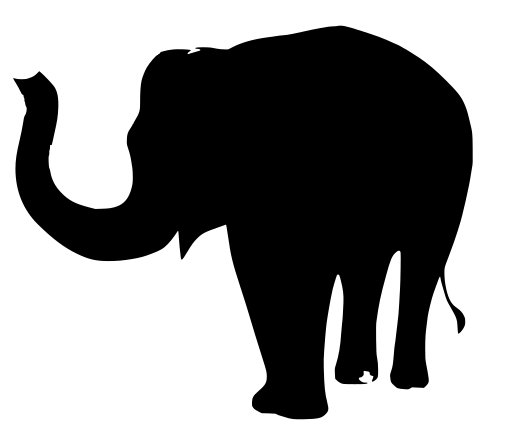
\includegraphics[width=0.5cm]{images/elephant.png}
	
}
%Note the empty line: without it will not yield what we want!!

\noindent After such a large gap, you should continue without indented first line! Most supervisors may find such embellishments distracting, unscientific bauble (and they are, but hey, life is also fun). So better check with them before submission!

%\clearpage
%
%{\Large \textbf{Want to write your BSc or MSc thesis under my supervision? Read this first!}}

\bigskip
\noindent For those few people whose work will be assessed by me (Carsten Dormann, Uni Freiburg), here are some general but personal thoughts on what makes a great piece of science.

I think of science as composed of (at least) two parts: \emph{handcraft} and \emph{intellect}. The handcraft is important to ``get things right''. It is what you (hopefully) learn to a large extent at university, from designing experiments, to various methods of collecting data, lab work, plotting, analysing, to writing it all up in a standardised (and thereby easily accessible) way. Handcraft includes issues such as reproducibility and publishing ethics.

\emph{Intellect} is where the actual ``science'' happens, it is the progress in understanding the world, the increase in knowledge, the broadening of the mind and the trimming down on possible ways things could interact. I see handcraft as the stuff that every baker has to do, too: get the dough set up tastily, have the right ingredients, the right temperature in the oven, a clean working surface, safe working conditions, etc. The baker also should work reproducibly (from day to day) and ``publish'' (read: sell) his/her results.

It is harder to describe what is a ``good'', intellectual science contribution. As first approximation, I think science is stuff that will still be correct in, say, 500 years. I am not against short-term benefits of science, don't get me wrong, but those are largely engineering, i.e. applying in exceedingly smart ways our \emph{current} knowledge to problem solving. There is no demeaning in calling an activity ``engineering'': it is of vital importance for all our societies, our everyday life and our future. It is (or at least can be) highly creative and responsible, challenging and demanding the highest level of intelligence. During engineering projects, a lot of still-valid-in-500-year-stuff is being produced, i.e. science is ``done''. 

In a science degree, however, this is not the typical approach to ``doing science''.\footnote{I am aware that many politicians think that this is how science \emph{should} be done, that science is only to directly benefit the university, the society, the economy. Also, I am aware that some thinkers (in a wider sense of the word) suggest that most actual science progress is serendipitous, and hence engineering is all we need. I just happen to disagree, possibly for selfish, stupid or conservative reasons.} 
Here, understanding the inner workings is the goal, not an application, or problem solving activity, however worthy. And the key (only?) approach that has over a few centuries proven useful for ``doing science'' is ``the Scientific Method''. This is based on a theoretical understanding, from which we derive hypotheses that are then tested.\footnote{If unfamiliar with the Scientific Method, do read it up on Wikipedia or alike. By all means, also read the criticism levelled at this approach. Keep in mind, though, that ``the hard sciences'' (physics, chemistry and friends) use this approach as their bread-and-butter epistemology. Don't reject it just because you don't like it or find it wanting for some reason. It has a very good track record!}

For a BSc, MSc or other scientific work, this has substantial consequences. First, it requires the author to lay out the \textbf{theory}. Without theory (or model or process understanding) one cannot derive (``deduce'') hypotheses. Into how much detail of said theory one has to go depends on the actual hypothesis to be tested. If your theory is that the moon was formed from the same material as the earth, and you want to test the hypothesis that thus the mineral composition is the same for both celestial bodies, well, I guess you can keep it short and focus on \emph{which} minerals you want to investigate and \emph{why those}. On the other hand, I would like to know what makes you want to test such a theory, and while you can simply cite some authority on the subject, it is better practice to recount the actual arguments and facts so far.

Next comes the formulation of hypotheses that could be used to test this theory. Obviously a good theory makes an awful lot of statements, so we cannot, in a lifetime, test all of them. Typically the department where you work determines which hypotheses you will test. (This sounds like a really stupid reason, but in real life a lot of things are really stupid.) And, luckily, it is actually not such a bad reason. Your department (or your supervisor's department) will have experience in a certain way of hypothesis-forming and -testing, will have certain lab facilities, data, collaborations, expeditions and so forth. Hence even though the best way to test a theory may be a specific hypothesis, it will simply be out of reach (think: explode a planet, fly at 90\% the speed of light or speak fluent Khoisan). It is IMHO extremely important to be aware of these constraints and limitations! You should be able to answer to any journalist with the best possible way to test a theory, and why you couldn't use that approach. Don't even pretend that your approach is anywhere near optimal or even decent. We all are aware of how limited our possibilities are, and grandiousing our ways (if that is a word) is silly, self-deceiving and transparently wrong.

It is very useful, and hard, to go through all the possible outcomes of your hypothesis-testing and work out \emph{in advance} what you learn from it. If there are 120 ways why you don't get a positive finding, well, then you don't actually learn much from such a negative finding. Since most easy hypotheses have been tested over the last few hundred years of science, you will most likely find your hypothesis rejected. That is, in itself, fine. But it is only fine if you still learn something from it, if it narrows down possibilities. If, say, you find that a higher plant species richness does \emph{not} lead to a higher monkey density in a Madagascan forest, well, there may be hundreds of reasons why it didn't. This is no intellectual progress. It is not the lack of a positive finding, it is the lack of a \emph{conclusive} negative finding that will bother reviewers! If, in contrast, you visited one of the 10 candidates for a meteorite impact crater responsible for the \href{https://en.wikipedia.org/wiki/Permian%E2%80%93Triassic_extinction_event}{Permian-Triassic extinction event}, 
and you found the isotop composition not to be consistent with this site being ``it'', well, then we actually learned something (for the next 500 years)!

Where, you may ask, was the ``intellect'' in the last example? Good point! That was indeed handcraft research, not intellectual science. Note that this is a document for BSc and MSc theses, not the Noble Price. And for a, say, MSc thesis I would be very happy to read the theoretical reasoning, the derivation of what to expect if this site \emph{were} the impact crater, to see the discussion (and quantification) of the uncertainty of the isotope measurements and thus the strength of the rejection of this site. It would, to me, demonstrate that you had worked scientifically. Would you get full marks? Alas, no. The missing bit was the curiousity driven, creative advancement to theory. Not everybody will be able to do that. In fact, I doubt that I have made substantial contributions to this still-valid-in-500-years-stuff (and I certainly never got full marks after leaving school). But that is exactly what a full marks means: exceptional, outstanding, dazzling! And few of us are geniuses worthy of full marks, sorry. You can become a good scientist, contributing to advancing the work on the still-valid-in-500-years-stuff even without being a genius (at least that's what I keep telling myself).

So I guess what I'm saying is: Don't expect exceedingly good marks from me.

